% Confirm-before-acting paper. Build: tectonic main.tex (or pdflatex + bibtex), or upload the folder to Overleaf.
% Every number in tables.tex and numbers.tex is written by make_paper.py from the result files;
% do not type numbers into this file by hand.
\documentclass[11pt]{article}
\usepackage[final]{acl}
\usepackage{times}
\usepackage{latexsym}
\usepackage[T1]{fontenc}
\usepackage[utf8]{inputenc}
\usepackage{microtype}
\usepackage{inconsolata}
\usepackage{booktabs}
\usepackage{graphicx}
\usepackage{xcolor}
\usepackage{adjustbox}

% Written by make_paper.py. Do not edit.
\newcommand{\NItemsAll}{840}
\newcommand{\NItems}{829}
\newcommand{\NSimple}{395}
\newcommand{\NMultiple}{196}
\newcommand{\NIrrelevance}{238}
\newcommand{\WerPhone}{1.6}
\newcommand{\WerNoiseTen}{2.0}
\newcommand{\WerNoiseZero}{6.5}
\newcommand{\WerChatterFive}{9.3}
\newcommand{\WerChatterZero}{48.9}
\newcommand{\TextsDifferMin}{63.6}
\newcommand{\TextsDifferMax}{79.6}
\newcommand{\HeadNever}{16.6}
\newcommand{\HeadEither}{5.8}
\newcommand{\HeadAsked}{20.7}
\newcommand{\QwenNeverMin}{14.8}
\newcommand{\QwenNeverMax}{20.7}
\newcommand{\QwenEitherMin}{5.1}
\newcommand{\QwenEitherMax}{6.0}
\newcommand{\QwenAskedMin}{20.1}
\newcommand{\QwenAskedMax}{25.3}
\newcommand{\QwenAccSaid}{82.4}
\newcommand{\QwenMissedMin}{22}
\newcommand{\QwenMissedMax}{30}
\newcommand{\QwenMissedChatter}{181}
\newcommand{\QwenBothMin}{4.2}
\newcommand{\QwenBothMax}{4.9}
\newcommand{\QwenBothAskedMin}{22.0}
\newcommand{\QwenBothAskedMax}{27.3}
\newcommand{\QwenSampAskedMin}{7.5}
\newcommand{\QwenSampAskedMax}{8.2}
\newcommand{\QwenQuestionMisheard}{5.8}
\newcommand{\LlamaNeverMin}{26.8}
\newcommand{\LlamaNeverMax}{33.2}
\newcommand{\LlamaEitherMin}{11.5}
\newcommand{\LlamaEitherMax}{13.3}
\newcommand{\LlamaAskedMin}{25.1}
\newcommand{\LlamaAskedMax}{34.5}
\newcommand{\LlamaAccSaid}{73.2}
\newcommand{\LlamaMissedMin}{0}
\newcommand{\LlamaMissedMax}{2}
\newcommand{\LlamaMissedChatter}{55}
\newcommand{\LlamaBothMin}{3.9}
\newcommand{\LlamaBothMax}{4.9}
\newcommand{\LlamaBothAskedMin}{42.9}
\newcommand{\LlamaBothAskedMax}{49.6}
\newcommand{\LlamaSampAskedMin}{35.1}
\newcommand{\LlamaSampAskedMax}{36.9}
\newcommand{\LlamaQuestionMisheard}{6.8}
\newcommand{\GainMin}{3.1}
\newcommand{\GainMax}{4.8}
\newcommand{\SigFiveQwen}{3}
\newcommand{\SigFiveLlama}{0}
\newcommand{\SigTenQwen}{4}
\newcommand{\SigTenLlama}{1}
\newcommand{\SigTwentyQwen}{4}
\newcommand{\SigTwentyLlama}{4}
\newcommand{\RealisedMin}{18.7}
\newcommand{\RealisedMax}{21.2}
\newcommand{\AlwaysMin}{55}
\newcommand{\AlwaysMax}{87}
\newcommand{\ChatterAskedMin}{33}
\newcommand{\ChatterAskedMax}{64}
\newcommand{\AgentWrongMin}{15}
\newcommand{\AgentWrongMax}{33}
\newcommand{\HearCausedMin}{9}
\newcommand{\HearCausedMax}{65}
\newcommand{\HearCausedChatMin}{72}
\newcommand{\HearCausedChatMax}{285}
\newcommand{\ScDiffMin}{$-$1.0}
\newcommand{\ScDiffMax}{$+$1.4}
\newcommand{\ScThirtyQwenVarBetter}{3}
\newcommand{\ScThirtyLlamaSig}{0}
\newcommand{\ScThirtyLlamaAheadMin}{0.2}
\newcommand{\ScThirtyLlamaAheadMax}{2.1}
\newcommand{\ScThirtyQwenAheadMin}{1.6}
\newcommand{\ScThirtyQwenAheadMax}{2.5}
\newcommand{\HearDiffMin}{0.5}
\newcommand{\HearDiffMax}{1.1}
\newcommand{\HearAllAhead}{10}
\newcommand{\HearSig}{5}
\newcommand{\HearN}{10}
\newcommand{\WordN}{96}
\newcommand{\WordBetter}{1}
\newcommand{\WordWorse}{4}
\newcommand{\WordMaxAbs}{2.5}
\newcommand{\WordBetterBy}{1.8}
\newcommand{\SigThirtyAll}{8}
\newcommand{\ScSigCount}{0}
\newcommand{\CatchHearMin}{90}
\newcommand{\CatchHearMax}{100}
\newcommand{\CatchHearUttMin}{30}
\newcommand{\CatchHearUttMax}{53}
\newcommand{\CatchAgentMin}{50}
\newcommand{\CatchAgentMax}{62}
\newcommand{\CatchAgentUttMin}{30}
\newcommand{\CatchAgentUttMax}{42}
\newcommand{\CostOneWrongMin}{11.8}
\newcommand{\CostOneWrongMax}{12.1}
\newcommand{\CostOneAskedMin}{5.8}
\newcommand{\CostOneAskedMax}{8.1}


\title{Read It Back When the Action Is Unstable:\\Confirmation Policies for Spoken Tool Calling}

\author{Masood Ahmed \\
  Independent researcher, Islamabad, Pakistan \\
  \texttt{masoodd.ahmedd123@gmail.com}}

\begin{document}
\maketitle

\begin{abstract}
A voice agent that calls tools can read an action back before doing it (``Area of a triangle, base 10, height 5, is that right?''). Confirming every action makes the agent tedious; confirming none lets it act on misheard words and on its own misreadings. Recent benchmarks measure how often speech recognition errors turn into wrong tool calls, but not which signal should decide when to ask. We compare confirmation policies on \NItems{} spoken requests from BFCL v3 audio, played clean, through a simulated phone line, and with environmental noise or background chatter, with Whisper as the recogniser and Qwen2.5-7B and Llama-3.1-8B as agents. Utterance-level recogniser confidence is a weak guide. A much better one is whether the agent's call changes when it is given the recogniser's other likely transcripts: confirming only those requests reduces wrong actions taken without asking from \HeadNever\% to \HeadEither\% of requests while asking on \HeadAsked\% (Qwen, phone line with 10 dB noise), and at a fixed 20\% confirmation budget it leaves \GainMin{} to \GainMax{} fewer wrong actions per 100 requests than utterance confidence, with 95\% intervals excluding zero for both agents in all four conditions without chatter. Most of the wrong actions it stops are not mishearings but the agent's own mistakes, and re-sampling the agent on a single transcript works about as well at the same budget. The useful signal is therefore the stability of the action under a small nudge, and combining both nudges leaves the fewest wrong actions. Under loud background chatter, where most requests are misheard, no policy keeps both wrong actions and confirmations low. Code and results are public.
\end{abstract}

\section{Introduction}

Spoken requests to a tool-calling agent fail in two ways. The recogniser can mishear (``fifteen'' for ``fifty''), and the agent can misread a request it heard correctly (the wrong function, a missing argument, a unit in the wrong place). Either way the agent takes a wrong action. The classical remedy from spoken dialogue systems is confirmation: read the action back and let the user say no \citep{sturm1999arise,bohus2005rejection}. Confirmation has a cost, since every read-back is a turn the user did not ask for, so a deployed agent needs a rule for \emph{when} to ask.

Recent work has made the size of the problem clear. Speech versions of function-calling benchmarks show that recognition errors cost several points of call accuracy, mostly through misheard argument values \citep{mao2026bfclaudio,wang2026speechevalx,laskar2026texttovoice,jain2025voiceagentbench}. These studies diagnose the failure; they do not test what an agent should do about it at run time. Text-only work on when an LLM should ask a clarifying question \citep{kuhn2022clam,zhang2025clarify,ross2025when2call,suri2026sage} does not see the recogniser at all.

We compare confirmation policies directly. Every policy decides, per request, whether to read the action back, and we score the trade-off between wrong actions taken without asking and the share of requests confirmed. We ask:
\begin{enumerate}
\item Which run-time signal best ranks requests for confirmation: recogniser confidence at the utterance, word or argument level, disagreement among transcript variants, or the agent's own self-consistency?
\item How much of the benefit comes from catching mishearings, and how much from catching the agent's own mistakes?
\item What does the better signal cost in extra agent calls, and where does it stop helping?
\end{enumerate}

Our main finding is that the most useful signal is not how sure the recogniser is but how stable the agent's action is. Giving the agent the recogniser's 5-best hypotheses and a second recogniser's transcript, and confirming whenever any of them changes the call, beats every recogniser-confidence ranking. It works mostly because it exposes calls the agent was guessing at, whatever the cause; re-sampling the agent on the same transcript exposes many of the same calls. We release the code, the per-request results and the scripts that write every number in this paper.\footnote{\url{https://github.com/masooddahmedd/confirm-before-acting}}

\section{Related work}

\paragraph{Spoken tool calling.} BFCL \citep{patil2025bfcl}, built on Gorilla \citep{patil2023gorilla}, scores function calls by matching their syntax trees against allowed values. BFCL Audio \citep{mao2026bfclaudio} evaluates pipelined and end-to-end audio function calling under accents, disfluencies and noise, and AU-Harness \citep{nguyen2025auharness} includes a spoken version of BFCL v3 as one of its tasks, which is the data we use. VoiceAgentBench \citep{jain2025voiceagentbench} covers spoken agentic queries in English and six Indic languages, \citet{laskar2026texttovoice} convert text tool benchmarks to noisy audio and find that most voice failures are misheard argument values, and \citet{wang2026speechevalx} show that edits to numbers and negations cost the most. Full-Duplex-Bench-v3 \citep{lin2026fullduplexbenchv3} adds real disfluent speech and chained calls. All of these measure the damage; we evaluate a run-time defence.

\paragraph{Confirmation in dialogue systems.} Classical systems chose between explicit, implicit and no confirmation from recogniser confidence \citep{sturm1999arise,bouwman1999confidence}, set confidence thresholds per dialogue state by weighing the cost of a wrong concept against an extra turn \citep{bohus2005rejection}, and studied recovery after non-understanding \citep{bohus2005sorry}. \citet{kim2021clarifying} train a model that decides when a voice assistant should ask a clarifying question. Confidence measures for recognition are surveyed by \citet{jiang2005confidence}, and n-best hypotheses are known to help spoken language understanding \citep{li2020nbest,ganesan2021nbest}. These systems predate LLM agents, whose own errors, as we show, outnumber the recogniser's.

\paragraph{Selective prediction and clarification for LLMs.} Selective classification trades coverage for error \citep{geifman2017selective,kamath2020selective}; a confirmation policy is the same trade with ``ask the user'' in place of ``abstain''. Agreement among samples is a strong signal of correctness \citep{wang2023selfconsistency}, and semantic entropy over sampled answers detects confabulation \citep{kuhn2023semantic,farquhar2024semanticentropy}. For tool use, When2Call \citep{ross2025when2call} tests whether a model should call, ask or decline, SAGE \citep{suri2026sage} asks when the expected value of a parameter's information is high, and ToolEmu \citep{ruan2024toolemu} shows that agents often take risky actions. Our transcript-variant signal is a cheap, recogniser-driven relative of sample agreement, and we compare the two directly.

\section{Setup}

\paragraph{Requests.} We use the spoken version of BFCL v3 distributed with AU-Harness \citep{nguyen2025auharness,servicenow2025bfclv3audio}: the \emph{simple}, \emph{multiple} and \emph{irrelevance} subsets, \NItemsAll{} requests with the function schemas and allowed argument values of the original benchmark. We drop clips longer than one 30-second Whisper window, leaving \NItems{} (\NSimple{} simple, \NMultiple{} with several candidate functions, \NIrrelevance{} where no function fits and the correct answer is no call). The audio is synthetic speech that paraphrases the written question, often with an extra sentence of context.

\paragraph{Listening conditions.} Each request is heard in six conditions: the clean audio; a phone line (band-pass 300--3400\,Hz, resampled to 8\,kHz, G.711 $\mu$-law \citep{itu1988g711}, back to 16\,kHz); the phone line with environmental noise from ESC-50 \citep{piczak2015esc} at 10\,dB and 0\,dB SNR; and the phone line with background chatter made of three other requests from the benchmark at 5\,dB and 0\,dB. Noise clips and talkers are drawn per request with a fixed seed.

\paragraph{Recognisers.} Whisper large-v3-turbo \citep{radford2023whisper}, run through faster-whisper and CTranslate2,\footnote{faster-whisper 1.2.1 and CTranslate2 4.8.2: \url{https://github.com/SYSTRAN/faster-whisper}.} with beam size 5, returns the top transcript, per-word probabilities, the utterance log-probability and its 5-best list. Whisper large-v3 gives a second, independent transcript. Word error rates against the clean-audio transcript are \WerPhone\% on the phone line, \WerNoiseTen\% and \WerNoiseZero\% with noise, and \WerChatterFive\% and \WerChatterZero\% with chatter (Appendix Table~\ref{tab:acc}).

\paragraph{Agents.} Qwen2.5-7B-Instruct \citep{qwen2024qwen25} and Llama-3.1-8B-Instruct \citep{grattafiori2024llama3}, served by Ollama\footnote{Ollama 0.11.4: \url{https://github.com/ollama/ollama}.} with greedy decoding, a fixed seed and JSON output. The system prompt (Appendix~\ref{app:prompt}) lists the request's function schemas and asks for a list of calls, or an empty list when no function fits. Calls are graded with a reimplementation of BFCL's AST checker: the right function, every required argument present with an allowed value, optional arguments absent or allowed, no unknown arguments, and no call at all for irrelevance requests. On the clean transcript Qwen is right on \QwenAccSaid\% of requests and Llama on \LlamaAccSaid\%.

\section{Confirmation policies and evaluation}

\paragraph{What a confirmation does.} If the agent calls nothing there is nothing to confirm. Otherwise a policy either acts or reads the call back. We simulate an ideal user who always rejects a wrong read-back and accepts a right one. Our main measure is the share of requests on which the agent \emph{takes a wrong action without asking}: a confirmed wrong action is stopped whatever caused it, and a confirmed right action costs one unnecessary turn. We report the confirmation rate next to it. Missed actions, where the agent calls nothing although a call was needed, cannot be fixed by confirming and are counted apart (Qwen \QwenMissedMin{} to \QwenMissedMax{} of \NItems{} without chatter, Llama \LlamaMissedMin{} to \LlamaMissedMax). A second, hearing-only measure replaces a confirmed action by the agent's action on the clean transcript, so that only mishearing counts as preventable (Appendix Table~\ref{tab:hearing}).

\paragraph{Which mistakes are mishearings.} Splitting wrong actions into mishearing and the agent's own mistakes needs a reference for what the user said. The benchmark's written question is the wrong reference: because the audio paraphrases it, using it marks \QwenQuestionMisheard\% (Qwen) and \LlamaQuestionMisheard\% (Llama) of requests on \emph{clean} audio as misheard. We use the clean-audio transcript instead. A wrong action is a mishearing if the agent's call on the clean transcript is right and its call on the degraded transcript is wrong; otherwise it is an agent mistake. The main measure does not depend on this choice.

\paragraph{Signals.} A policy confirms requests whose signal is high.
\begin{itemize}
\item \textbf{Utterance confidence}: the negative average log-probability of the top transcript.
\item \textbf{Lowest word confidence}: one minus the smallest word probability.
\item \textbf{Argument-word confidence}: one minus the smallest probability among transcript words that appear in the call's argument values.
\item \textbf{Transcript variants}: the agent is also run on each distinct 5-best hypothesis and on the second recogniser's transcript; the signal is whether, and how many of, these calls differ from the call on the top transcript, compared after normalising strings and numbers.
\item \textbf{Agent samples (self-consistency)}: the agent answers the top transcript 4 more times at temperature 0.7 with fixed seeds; the signal is whether any sample's call differs from the greedy call.
\end{itemize}
Disagreement signals are nearly yes/no, so we report them in two forms: as a yes/no rule at its own confirmation rate, and as a ranked policy that puts every disagreeing request first and breaks ties by argument-word confidence, so it can be held to a budget.

\paragraph{Budgets and inference.} Ranked policies are held to confirmation budgets of 5, 10, 20 and 30\% of requests. To avoid tuning on the requests being scored, requests are split in two halves by a hash of their id; the threshold for a budget is chosen on one half and applied to the other, in both directions, so that every request gets exactly one out-of-sample decision. We compare policies with 95\% paired bootstrap intervals over requests (2{,}000 resamples).

\section{Results}

\begin{table*}[t]\centering\small
\begin{adjustbox}{max width=\linewidth}\begin{tabular}{llrrrrr}\toprule
 & & & & \multicolumn{3}{c}{20\% confirmation budget} \\ \cmidrule(lr){5-7}
Agent & Condition & Never & Any variant disagrees & Utterance conf. & Variants, then arg. conf. & Difference [95\% CI] \\
\midrule
Qwen2.5-7B & clean & 14.8 & \textbf{5.1} (21.8) & 10.0 & 6.4 & $-$3.6 [$-$5.4, $-$1.7] \\
Qwen2.5-7B & phone & 15.6 & \textbf{5.8} (20.1) & 10.9 & 6.4 & $-$4.5 [$-$6.3, $-$2.5] \\
Qwen2.5-7B & noise 10 dB & 16.6 & \textbf{5.8} (20.7) & 11.2 & 6.4 & $-$4.8 [$-$6.8, $-$3.0] \\
Qwen2.5-7B & noise 0 dB & 20.7 & \textbf{6.0} (25.3) & 12.3 & 8.4 & $-$3.9 [$-$5.5, $-$2.1] \\
Qwen2.5-7B & chatter 5 dB & 22.2 & \textbf{4.1} (32.6) & 13.1 & 9.7 & $-$3.5 [$-$5.5, $-$1.7] \\
Qwen2.5-7B & chatter 0 dB & 32.0 & \textbf{2.2} (40.7) & 16.2 & 15.3 & $-$0.8 [$-$3.4, $+$1.8] \\
\midrule
Llama-3.1-8B & clean & 26.8 & \textbf{12.2} (27.9) & 19.4 & 15.2 & $-$4.2 [$-$6.5, $-$1.8] \\
Llama-3.1-8B & phone & 27.3 & \textbf{12.8} (26.2) & 19.2 & 15.9 & $-$3.3 [$-$5.5, $-$0.8] \\
Llama-3.1-8B & noise 10 dB & 28.3 & \textbf{13.3} (25.1) & 19.5 & 16.3 & $-$3.3 [$-$5.5, $-$0.8] \\
Llama-3.1-8B & noise 0 dB & 33.2 & \textbf{11.5} (34.5) & 22.3 & 19.2 & $-$3.1 [$-$5.2, $-$1.3] \\
Llama-3.1-8B & chatter 5 dB & 35.0 & \textbf{9.9} (39.9) & 22.7 & 20.7 & $-$1.9 [$-$4.1, $+$0.1] \\
Llama-3.1-8B & chatter 0 dB & 56.6 & \textbf{4.2} (63.8) & 39.2 & 37.9 & $-$1.3 [$-$4.0, $+$1.5] \\
\bottomrule\end{tabular}\end{adjustbox}
\caption{Wrong actions taken without asking (\% of 829 requests). \emph{Never}: the agent always acts. \emph{Any variant disagrees}: confirm when the call from any of the 5-best transcripts or the second recogniser differs from the call on the top transcript; its confirmation rate in brackets. The two ranked policies are held to a 20\% confirmation budget with cross-fitted thresholds (realised rates 18.7--21.2\%). Difference: ranked variant policy minus utterance confidence, in points, with a 95\% paired bootstrap interval.}\label{tab:main}
\end{table*}

\begin{table}[t]\centering\small\setlength{\tabcolsep}{4pt}
\begin{adjustbox}{max width=\linewidth}\begin{tabular}{llrrrrr}\toprule
 & & & \multicolumn{2}{c}{Mishearing} & \multicolumn{2}{c}{Agent} \\ \cmidrule(lr){4-5}\cmidrule(lr){6-7}
Agent & Cond. & Asked & Var. & Utt. & Var. & Utt. \\ \midrule
Qwen2.5 & phone & 20.1 & 9/9 & 3/9 & 72/120 & 36/120 \\
Qwen2.5 & noise 10 dB & 20.7 & 16/17 & 9/17 & 74/121 & 36/121 \\
Qwen2.5 & noise 0 dB & 25.3 & 50/55 & 41/55 & 72/117 & 43/117 \\
Qwen2.5 & chatter 5 dB & 32.6 & 69/72 & 61/72 & 81/112 & 50/112 \\
Qwen2.5 & chatter 0 dB & 40.7 & 175/184 & 163/184 & 72/81 & 65/81 \\
\midrule
Llama & phone & 26.2 & 10/10 & 3/10 & 110/216 & 77/216 \\
Llama & noise 10 dB & 25.1 & 18/20 & 10/20 & 107/215 & 75/215 \\
Llama & noise 0 dB & 34.5 & 60/65 & 48/65 & 120/210 & 89/210 \\
Llama & chatter 5 dB & 39.9 & 81/85 & 70/85 & 127/205 & 96/205 \\
Llama & chatter 0 dB & 63.8 & 272/285 & 262/285 & 162/184 & 148/184 \\
\bottomrule\end{tabular}\end{adjustbox}
\caption{Which wrong actions each signal catches at the same number of confirmations. Mishearing: the agent's call on the clean-audio transcript is right but the call on the degraded one is wrong. Agent: the call is wrong on the clean transcript too. Var.: any variant disagrees; Utt.: utterance confidence at the same rate.}\label{tab:catch}
\end{table}

\begin{table}[t]\centering\small\setlength{\tabcolsep}{4pt}
\begin{adjustbox}{max width=\linewidth}\begin{tabular}{lrrrrr}\toprule
 & & \multicolumn{2}{c}{Qwen2.5-7B} & \multicolumn{2}{c}{Llama-3.1-8B} \\ \cmidrule(lr){3-4}\cmidrule(lr){5-6}
Variants checked & Calls & Asked & Wrong & Asked & Wrong \\ \midrule
none & 0 & 0.0 & 16.6 & 0.0 & 28.3 \\
second recogniser & 1 & 5.8 & 12.1 & 7.6 & 22.2 \\
2nd beam hypothesis & 1 & 8.1 & 11.8 & 8.6 & 22.2 \\
beam hypotheses 2--3 & 2 & 13.5 & 8.9 & 16.8 & 16.9 \\
beam hypotheses 2--5 & 4 & 20.0 & 6.3 & 24.6 & 13.5 \\
5-best + second recogniser & 5 & 20.7 & 5.8 & 25.1 & 13.3 \\
\bottomrule\end{tabular}\end{adjustbox}
\caption{Cost: extra agent calls per request against wrong actions taken without asking (\%), noise 10 dB. The rule confirms when any checked variant changes the call.}\label{tab:cost}
\end{table}

\begin{table*}[t]\centering\small
\setlength{\tabcolsep}{4pt}\begin{adjustbox}{max width=\linewidth}\begin{tabular}{llrrrrrrr}\toprule
 & & \multicolumn{3}{c}{Yes/no rule: confirm when \dots\ disagree} & \multicolumn{3}{c}{20\% budget} & 30\% budget \\ \cmidrule(lr){3-5}\cmidrule(lr){6-8}\cmidrule(lr){9-9}
Agent & Cond. & samples & beam 2--5 & either & Var. & Samp. & Samp.$-$var. & Samp.$-$var. \\ \midrule
Qwen2.5 & clean & 10.1 {\scriptsize (7.5)} & 5.4 {\scriptsize (21.0)} & 4.2 {\scriptsize (23.5)} & 6.4 & 7.4 & $+$1.0 {\scriptsize [$-$0.6, $+$2.5]} & $+$1.1 {\scriptsize [$-$0.4, $+$2.4]} \\
Qwen2.5 & phone & 10.4 {\scriptsize (7.7)} & 6.2 {\scriptsize (19.5)} & 4.9 {\scriptsize (22.0)} & 6.4 & 7.6 & $+$1.2 {\scriptsize [$-$0.5, $+$2.8]} & $+$1.6 {\scriptsize [$+$0.2, $+$2.9]} \\
Qwen2.5 & noise 10 dB & 11.8 {\scriptsize (8.2)} & 6.3 {\scriptsize (20.0)} & 4.9 {\scriptsize (22.3)} & 6.4 & 7.8 & $+$1.4 {\scriptsize [$-$0.2, $+$3.0]} & $+$1.6 {\scriptsize [$+$0.2, $+$3.0]} \\
Qwen2.5 & noise 0 dB & 15.3 {\scriptsize (8.0)} & 7.4 {\scriptsize (23.5)} & 4.9 {\scriptsize (27.3)} & 8.4 & 9.0 & $+$0.6 {\scriptsize [$-$1.2, $+$2.3]} & $+$2.5 {\scriptsize [$+$0.8, $+$4.1]} \\
\midrule
Llama & clean & 7.0 {\scriptsize (35.2)} & 12.4 {\scriptsize (27.1)} & 3.9 {\scriptsize (45.6)} & 15.2 & 14.7 & $-$0.5 {\scriptsize [$-$2.4, $+$1.3]} & $-$1.6 {\scriptsize [$-$3.7, $+$0.6]} \\
Llama & phone & 6.8 {\scriptsize (35.7)} & 13.3 {\scriptsize (25.2)} & 4.3 {\scriptsize (43.9)} & 15.9 & 15.4 & $-$0.5 {\scriptsize [$-$2.4, $+$1.3]} & $-$2.1 {\scriptsize [$-$4.3, $+$0.1]} \\
Llama & noise 10 dB & 8.1 {\scriptsize (35.1)} & 13.5 {\scriptsize (24.6)} & 4.9 {\scriptsize (42.9)} & 16.3 & 15.6 & $-$0.7 {\scriptsize [$-$2.8, $+$1.2]} & $-$1.4 {\scriptsize [$-$3.6, $+$0.6]} \\
Llama & noise 0 dB & 9.9 {\scriptsize (36.9)} & 12.9 {\scriptsize (32.4)} & 4.3 {\scriptsize (49.6)} & 19.2 & 18.2 & $-$1.0 {\scriptsize [$-$3.1, $+$1.1]} & $-$0.2 {\scriptsize [$-$2.4, $+$1.9]} \\
\bottomrule\end{tabular}\end{adjustbox}
\caption{Transcript variants against agent self-consistency (4 samples at temperature 0.7 on the top transcript), wrong actions taken without asking (\%), confirmation rate in brackets. Samples and beam hypotheses 2--5 cost the same 4 extra calls; \emph{either} confirms when any transcript variant or any sample disagrees. The budget columns rank by disagreement (Var.: transcript variants; Samp.: samples), break ties by argument-word confidence, and give the difference in points with a 95\% paired bootstrap interval (at 30\%, the difference only).}\label{tab:sc}
\end{table*}



\begin{figure*}[t]\centering
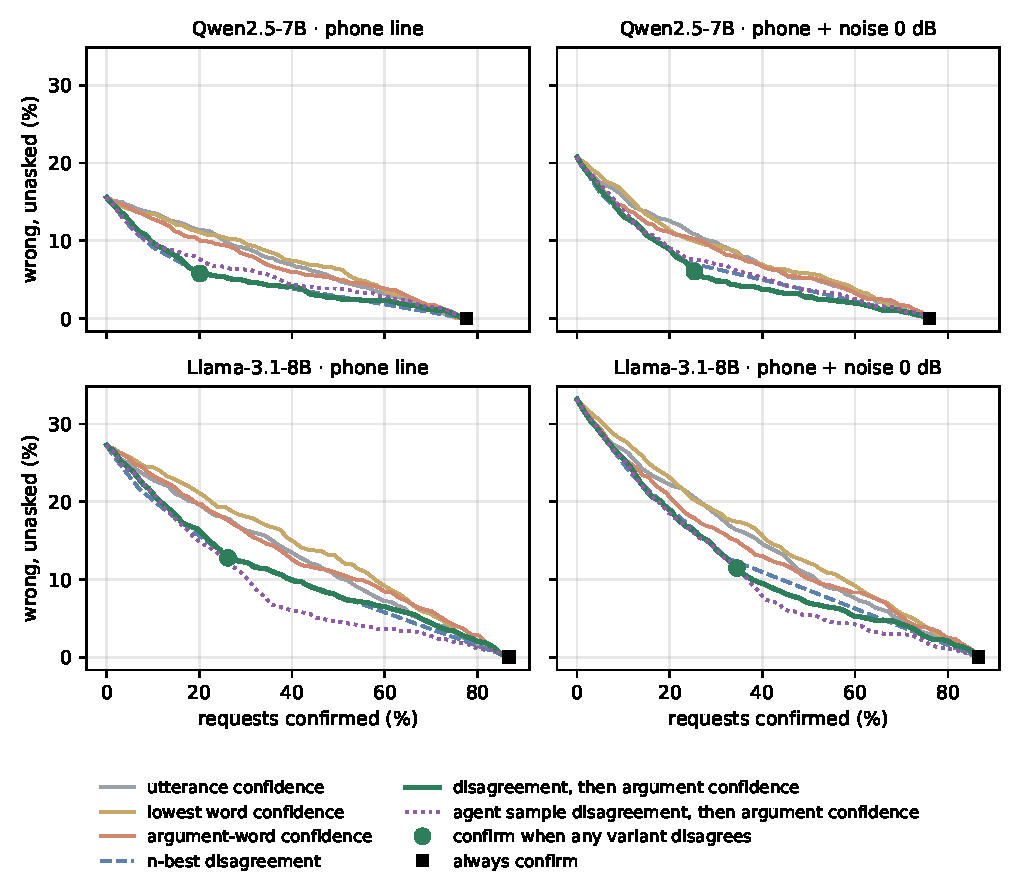
\includegraphics[width=0.86\textwidth]{fig_tradeoff.pdf}
\caption{Wrong actions taken without asking against requests confirmed, as the threshold of each ranked policy sweeps over all requests (descriptive, not cross-fitted). Dot: confirm when any transcript variant disagrees. Square: confirm every action.}\label{fig:tradeoff}
\end{figure*}

\paragraph{Transcript variants beat recogniser confidence.} Table~\ref{tab:main} gives the main result. Without confirmation the agents act wrongly on \QwenNeverMin--\QwenNeverMax\% (Qwen) and \LlamaNeverMin--\LlamaNeverMax\% (Llama) of requests in the four conditions without chatter. Confirming when any transcript variant changes the call brings this down to \QwenEitherMin--\QwenEitherMax\% at \QwenAskedMin--\QwenAskedMax\% asked for Qwen, and to \LlamaEitherMin--\LlamaEitherMax\% at \LlamaAskedMin--\LlamaAskedMax\% asked for Llama. Held to a 20\% budget (realised \RealisedMin--\RealisedMax\%), the ranked variant policy leaves \GainMin{} to \GainMax{} fewer wrong actions per 100 requests than utterance confidence, and the interval excludes zero for both agents in all four conditions. The gap needs some budget: at 5\% the variant policy is reliably better for Qwen in \SigFiveQwen{} of the 4 conditions and for Llama in \SigFiveLlama, at 10\% in \SigTenQwen{} and \SigTenLlama, and at 20\% and 30\% in all four for both. Figure~\ref{fig:tradeoff} shows the whole trade-off. Confirming everything removes all wrong actions but asks on \AlwaysMin--\AlwaysMax\% of requests.

The word-level signals are no improvement on the utterance. Ranking by the lowest word probability or by the probability of the words that end up in the arguments stays within \WordMaxAbs{} points of utterance confidence; over \WordN{} comparisons (2 agents, 6 conditions, 2 signals, 4 budgets) it is reliably better \WordBetter{} time, by \WordBetterBy{} points, and reliably worse \WordWorse{} times.

\paragraph{Why it works: most wrong actions are the agent's.} Without chatter, only \HearCausedMin{} to \HearCausedMax{} of \NItems{} requests per degraded condition go wrong because of the audio, while the agent acts wrongly on \AgentWrongMin--\AgentWrongMax\% of all requests (Table~\ref{tab:catch}). At the same number of confirmations, transcript variants catch \CatchHearMin--\CatchHearMax\% of the mishearing-caused wrong actions on the phone line and with 10\,dB noise, against \CatchHearUttMin--\CatchHearUttMax\% for utterance confidence. More importantly, they also catch \CatchAgentMin--\CatchAgentMax\% of the agent's own mistakes, against \CatchAgentUttMin--\CatchAgentUttMax\%. A variant usually differs from the top transcript in a small way (``ten'' for ``10'', a comma, one function word). When such a change flips the call, the agent was not reading the request robustly, and the call is often wrong even on the clean transcript. Under the hearing-only measure, which gives no credit for catching the agent's mistakes, the room to improve is small; the variant policy is still ahead of utterance confidence at 20\% in all \HearN{} degraded conditions, by \HearDiffMin{} to \HearDiffMax{} points, reliably in \HearSig{} (Appendix Table~\ref{tab:hearing}).

\paragraph{Cost.} Each variant is an extra agent call. The calls are independent and can run in parallel, so latency stays close to one call, but compute grows. Table~\ref{tab:cost} shows that one extra call already helps: the second recogniser alone or the second beam hypothesis alone cuts Qwen's wrong actions from \HeadNever\% to \CostOneWrongMin--\CostOneWrongMax\% at \CostOneAskedMin--\CostOneAskedMax\% asked, and most of the full benefit arrives with four beam hypotheses. Across conditions at least one variant differs as text from the top transcript on \TextsDifferMin--\TextsDifferMax\% of requests without chatter, but most such differences do not change the call; only those that do trigger a confirmation.

\paragraph{Transcript variants against self-consistency.} If the variants mainly expose unstable calls, any perturbation of the agent might do. Table~\ref{tab:sc} tests this with the same budget of 4 extra calls. At a 20\% budget the two nudges are not reliably different for either agent in any condition (differences \ScDiffMin{} to \ScDiffMax{} points). At 30\% they part ways by agent: for Qwen the transcript variants are reliably ahead in \ScThirtyQwenVarBetter{} of 4 conditions, by \ScThirtyQwenAheadMin{} to \ScThirtyQwenAheadMax{} points, while for Llama the samples are ahead by \ScThirtyLlamaAheadMin{} to \ScThirtyLlamaAheadMax{} points, never reliably. The agents differ mainly in how often their samples disagree: Qwen's on only \QwenSampAskedMin--\QwenSampAskedMax\% of requests, Llama's on \LlamaSampAskedMin--\LlamaSampAskedMax\%. A nearly deterministic agent therefore gets little from re-sampling, and the transcript variants, which fire on a similar share of requests for both agents, are the more predictable choice. The two nudges catch partly different calls: confirming when either disagrees leaves the fewest wrong actions of any rule we test, \QwenBothMin--\QwenBothMax\% for Qwen at \QwenBothAskedMin--\QwenBothAskedMax\% asked and \LlamaBothMin--\LlamaBothMax\% for Llama at \LlamaBothAskedMin--\LlamaBothAskedMax\% asked.

\paragraph{Background chatter.} Chatter is where the picture changes. At 0\,dB the recogniser's word error rate is \WerChatterZero\%, mishearing causes \HearCausedChatMin{} to \HearCausedChatMax{} wrong actions per condition, and the agent finds no fitting function far more often (\QwenMissedChatter{} missed actions for Qwen, \LlamaMissedChatter{} for Llama). The yes/no variant rule still stops almost every wrong action, but it has to ask on \ChatterAskedMin--\ChatterAskedMax\% of requests. Held to 20\%, the variant policy is reliably better than utterance confidence only for Qwen at 5\,dB; in this regime recogniser confidence is itself a fair guide, catching most mishearing-caused wrong actions (Table~\ref{tab:catch}).

\section{Discussion}

For a practitioner the result is a simple recipe. Run the agent on the top transcript and on one or more alternatives, either the recogniser's next beam hypotheses or a second recogniser, and read the action back when the calls disagree. If the agent's sampling is noisy, sampled answers are a comparable signal, and the union of both is better still. Recogniser confidence alone is the weakest of the signals we test unless the audio is very poor.

The finding also changes what ``confirmation'' is for. Classical policies treated it as a defence against the recogniser \citep{sturm1999arise,bohus2005rejection}. With an LLM in the loop, most wrong actions on reasonable audio are the agent's, and a read-back is just as useful against those. Disagreement among nudged inputs is a cheap way to find them, close in spirit to self-consistency \citep{wang2023selfconsistency} but driven by the uncertainty the recogniser already exposes.

\section{Limitations}

The benchmark speech is synthetic; real callers hesitate, correct themselves and talk over noise, which should make mishearing more common than here. The simulated user always rejects a wrong read-back; real users sometimes accept one, which would shrink every policy's benefit, though not obviously their ranking. A rejected action is counted as stopped, not as fixed; the agent still has to get it right on the next turn. Requests are single-turn, English, and need at most a few calls. We test two 7--8B open agents; stronger agents make fewer mistakes of their own, so a larger share of their wrong actions would come from mishearing, where recogniser confidence does better. Self-consistency was run on the four conditions without chatter only, with one temperature and 4 samples. Thresholds are cross-fitted, but the set of signals, the tie-breaking rule and the budgets were chosen while looking at results on all requests, and the curves in Figure~\ref{fig:tradeoff} are descriptive. Under loud chatter no policy keeps both wrong actions and confirmations low; there the fix is a better recogniser, not a better rule for asking.

\section{Conclusion}

When a voice agent should read an action back is better decided by how stable its action is than by how confident its recogniser is. Checking whether the call survives the recogniser's alternative transcripts, or a few sampled answers, stops most wrong actions while asking on about a fifth to a third of requests, and it beats recogniser confidence at the same budget because most wrong actions on reasonable audio are the agent's own. Speech benchmarks for agents should report the wrong-action and confirmation trade-off, not only call accuracy.

\section*{Use of AI}
Experiments were run and this manuscript was drafted with the help of an AI coding assistant; every number in the paper is generated by the released scripts from the released result files, and the author is responsible for the content.

\bibliography{references}

\appendix
\section{Agent prompt}
\label{app:prompt}
\begin{quote}\small
You are a voice assistant that acts by calling functions. The user's words come from a speech recogniser.\\[2pt]
Available functions (JSON schema):\\
\textit{\{the request's function schemas\}}\\[2pt]
Reply with JSON only, in this exact shape:\\
\texttt{\{"calls": [\{"name": "<function name>", "arguments": \{<argument>: <value>\}\}]\}}\\
Use only the functions above and only arguments in their schemas, with values of the right type.
If none of the functions fits the request, reply \texttt{\{"calls": []\}}.
\end{quote}

\section{Additional tables}
Table~\ref{tab:acc} gives the recogniser's word error rate, how often the transcript variants differ as text, and the agents' call accuracy and error counts per condition. Table~\ref{tab:hearing} repeats the main comparison under the hearing-only measure.

\begin{table*}[t]\centering\small
\begin{adjustbox}{max width=\linewidth}\begin{tabular}{lrrrrrr}\toprule
 & clean & phone & noise 10 dB & noise 0 dB & chatter 5 dB & chatter 0 dB \\ \midrule
WER vs.\ clean transcript & -- & 1.6 & 2.0 & 6.5 & 9.3 & 48.9 \\
Any transcript variant differs & 66.1 & 63.6 & 67.9 & 79.6 & 88.5 & 98.6 \\
Qwen2.5-7B call accuracy & 82.4 & 81.5 & 80.7 & 75.6 & 74.3 & 46.2 \\
Llama-3.1-8B call accuracy & 73.2 & 72.7 & 71.7 & 66.6 & 64.5 & 36.8 \\
Qwen2.5-7B wrong actions / mishearing-caused & 123 / 0 & 129 / 9 & 138 / 17 & 172 / 55 & 184 / 72 & 265 / 184 \\
Llama-3.1-8B wrong actions / mishearing-caused & 222 / 0 & 226 / 10 & 235 / 20 & 275 / 65 & 290 / 85 & 469 / 285 \\
\bottomrule\end{tabular}\end{adjustbox}
\caption{Recogniser and agent per condition (\%). WER of Whisper large-v3-turbo against its own clean-audio transcript. Call accuracy is BFCL AST accuracy of the call on the top transcript.}\label{tab:acc}
\end{table*}

\begin{table*}[t]\centering\small
\begin{adjustbox}{max width=\linewidth}\begin{tabular}{llrrrrr}\toprule
 & & & & \multicolumn{3}{c}{20\% confirmation budget} \\ \cmidrule(lr){5-7}
Agent & Condition & Never & Any variant disagrees & Utterance conf. & Variants, then arg. conf. & Difference [95\% CI] \\ \midrule
Qwen2.5-7B & phone & 15.6 & 14.5 (20.1) & 15.2 & 14.5 & $-$0.7 [$-$1.3, $-$0.2] \\
Qwen2.5-7B & noise 10 dB & 16.6 & 14.7 (20.7) & 15.6 & 14.7 & $-$0.8 [$-$1.6, $-$0.2] \\
Qwen2.5-7B & noise 0 dB & 20.7 & 14.7 (25.3) & 16.2 & 15.1 & $-$1.1 [$-$2.2, $-$0.1] \\
Qwen2.5-7B & chatter 5 dB & 22.2 & 13.9 (32.6) & 16.6 & 16.0 & $-$0.6 [$-$1.9, $+$0.6] \\
Qwen2.5-7B & chatter 0 dB & 32.0 & 10.9 (40.7) & 20.3 & 19.7 & $-$0.6 [$-$2.8, $+$1.6] \\
\midrule
Llama-3.1-8B & phone & 27.3 & 26.1 (26.2) & 27.0 & 26.4 & $-$0.6 [$-$1.2, $-$0.1] \\
Llama-3.1-8B & noise 10 dB & 28.3 & 26.2 (25.1) & 27.4 & 26.7 & $-$0.7 [$-$1.4, $-$0.1] \\
Llama-3.1-8B & noise 0 dB & 33.2 & 25.9 (34.5) & 28.2 & 27.5 & $-$0.7 [$-$1.8, $+$0.2] \\
Llama-3.1-8B & chatter 5 dB & 35.0 & 25.2 (39.9) & 29.0 & 28.3 & $-$0.6 [$-$1.9, $+$0.6] \\
Llama-3.1-8B & chatter 0 dB & 56.6 & 23.8 (63.8) & 44.3 & 43.8 & $-$0.5 [$-$2.7, $+$1.7] \\
\bottomrule\end{tabular}\end{adjustbox}
\caption{The hearing-only measure: a confirmed action is replaced by the agent's action on the clean-audio transcript, so only mishearing counts as preventable (\%).}\label{tab:hearing}
\end{table*}


\end{document}
